\documentclass[11pt]{article}
\usepackage[utf8]{inputenc}
\usepackage[T1]{fontenc}
\usepackage[spanish,es-noshorthands]{babel}
\usepackage[margin=2.5cm]{geometry}
\usepackage{hyperref}
\hypersetup{colorlinks=true, linkcolor=blue, urlcolor=blue, citecolor=blue}
\usepackage{titlesec}
\usepackage{enumitem}
\usepackage{booktabs}
\usepackage{array}
\usepackage{tabularx}
\usepackage{parskip}
\usepackage{graphicx}
\usepackage{float}
\usepackage{caption}
\usepackage{amsmath}
\usepackage{textcomp}
\usepackage{tikz}
\usetikzlibrary{shapes.geometric, arrows.meta, positioning}

\titleformat{\section}{\large\bfseries}{\thesection}{1em}{}
\titleformat{\subsection}{\normalsize\bfseries}{\thesubsection}{1em}{}
\newcolumntype{Y}{>{\raggedright\arraybackslash}X}
\graphicspath{{img/}}

\title{\textbf{Informe Final \\ Ética y Seguridad de Datos (DS3031) -- Tipo 1}\\
\large Alzace Fitness: seguimiento de entrenamiento con privacidad diferencial}
\author{Joel M. Cayllahua Hilario \and Josué Renzo Hernández Yataco}
\date{\today}

\begin{document}
\maketitle

\begin{center}
\small Código: \url{https://github.com/Josu31506/Proyecto-2---etica-y-seguridad-de-datos}
\end{center}

\setcounter{tocdepth}{1}
\tableofcontents
\newpage

% ---------------------------------------------------------------
\section{Resumen}

Construimos una aplicación web para que Alzace Fitness acompañe a sus clientes de entrenamiento virtual. El cliente y su entrenador ven la ficha individual: mediciones, metas y sesiones. El club, en cambio, solo puede publicar una \textbf{estadística grupal protegida con privacidad diferencial}: los minutos activos promedio por persona y por mes.

Tres resultados principales:
\begin{itemize}[nosep]
  \item \textbf{Privacidad diferencial con $\varepsilon = 1$ por publicación.} En los datos de Fitbit, el error absoluto medio fue de \textbf{4,7 minutos} sobre una referencia de 34,05 min/día, y se devolvió un resultado en el 100\,\% de las 300 simulaciones. Elegimos $\varepsilon = 1$ porque es el menor valor ensayado que cumple el objetivo fijado de antemano: error medio $\le 5$ minutos y al menos 95\,\% de respuestas.
  \item \textbf{Costo en el modelo.} Al entrenar un clasificador con ruido de Laplace ($\varepsilon = 1$), la exactitud bajó de \textbf{70,9\,\% a 68,4\,\%} ($-2{,}5$ puntos). La caída fue algo mayor en el grupo femenino ($-3{,}1$) que en el masculino ($-2{,}0$).
  \item \textbf{Riesgo residual.} La DPIA identifica 9 riesgos a lo largo del ciclo de vida del dato. Después de las medidas implementadas, ninguno queda en nivel alto. Antes de un piloto con clientes reales quedan pendientes el despliegue con TLS y la definición de los plazos de conservación (sección~\ref{sec:cumplimiento}).
\end{itemize}

% ---------------------------------------------------------------
\section{Caso de negocio y KPIs}

Alzace Fitness pasa del entrenamiento presencial al virtual. Para no perder la supervisión, necesita registrar el progreso de cada cliente a distancia. Eso implica tratar \textbf{datos de salud} (frecuencia cardíaca, peso, grasa corporal y actividad), que la Ley N.\textdegree{}~29733 considera \textbf{datos sensibles}.

Los KPIs propuestos en el parcial se implementaron en el panel (tabla~\ref{tab:kpis}).

\begin{table}[H]
\centering\small
\begin{tabularx}{\textwidth}{@{}p{4.2cm}Y@{}}
\toprule
\textbf{KPI} & \textbf{Cómo se calcula en la aplicación} \\
\midrule
Adherencia al plan & Sesiones de la semana marcadas como cumplidas entre sesiones programadas. \\
Progreso hacia la meta & Combinación de la fracción de minutos alcanzada y la reducción de grasa desde la primera medición del periodo. El entrenador fija los pesos y cada componente va de 0 a 100\,\%. \\
Retención & Membresías activas al inicio de un mes cerrado que siguen activas al final. \\
Tiempo de respuesta ante alertas & Tiempo medio del mes entre que se activa una alerta por sesión pendiente y su primera atención. \\
\bottomrule
\end{tabularx}
\caption{KPIs del caso de negocio.}
\label{tab:kpis}
\end{table}

La estadística grupal protegida responde a una necesidad distinta: que el club conozca la tendencia de actividad de sus clientes \textbf{sin} poder reconstruir la rutina de ninguno de ellos.

% ---------------------------------------------------------------
\section{Datos}

\begin{table}[H]
\centering\small
\begin{tabularx}{\textwidth}{@{}p{3.3cm}YY@{}}
\toprule
\textbf{Dataset} & \textbf{Contenido} & \textbf{Uso en el proyecto} \\
\midrule
\href{https://www.kaggle.com/datasets/arashnic/fitbit}{Fitbit Fitness Tracker Data} & 33 participantes y 940 días-persona de actividad diaria, del 12 de abril al 12 de mayo de 2016. & Estadística protegida con privacidad diferencial y su experimento de utilidad. \\
\href{https://www.kaggle.com/datasets/valakhorasani/gym-members-exercise-dataset}{Gym Members Exercise} & 973 perfiles con edad, género, experiencia, frecuencia, duración de sesión, etc. & Modelo de clasificación con y sin protección, y análisis de sesgo. \\
\bottomrule
\end{tabularx}
\caption{Fuentes de datos.}
\end{table}

\textbf{Decisiones sobre los datos:}
\begin{itemize}[nosep]
  \item \textbf{Usamos solo la exportación de abril--mayo de Fitbit.} La exportación anterior (marzo--abril) tiene fechas solapadas con valores contradictorios. La importación verifica conflictos y se detiene si los encuentra.
  \item \textbf{Abandonamos el vínculo aleatorio Fitbit--Gym propuesto en el parcial.} Las fuentes no comparten un identificador de persona, así que unirlas al azar produciría ``clientes'' que no existen y conclusiones sin validez. Cada fuente se analiza por separado (sección~\ref{sec:lecciones}).
  \item \textbf{El identificador de Fitbit se seudonimiza} con HMAC-SHA-256 y una clave independiente antes de guardarse. Las identidades de la demo son ficticias.
\end{itemize}

\begin{figure}[H]
\centering
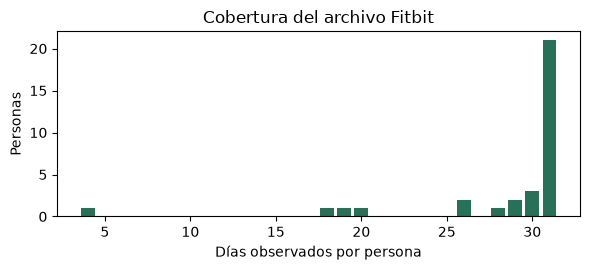
\includegraphics[width=0.75\textwidth]{cobertura-fitbit.png}
\caption{Días observados por persona en Fitbit. La mayoría tiene entre 28 y 31 días, pero algunas personas registran muy pocos (mínimo 4). Promediar por fila haría que las personas con más días pesen más; por eso la estadística da un voto a cada persona.}
\label{fig:cobertura}
\end{figure}

% ---------------------------------------------------------------
\section{Implementación}

\begin{table}[H]
\centering\small
\begin{tabularx}{\textwidth}{@{}p{2.4cm}p{3.6cm}Y@{}}
\toprule
\textbf{Capa} & \textbf{Tecnología} & \textbf{Qué hace} \\
\midrule
Frontend & Next.js & Pantallas separadas para Cliente (actividad, historial, importar CSV, privacidad), Entrenador (clientes asignados, metas, sesiones, alertas) y Administrador (estadísticas, auditoría, operaciones). \\
Backend & FastAPI (Python) & Autorización por rol y por registro, cifrado, privacidad diferencial, presupuesto $\varepsilon$, auditoría y respaldos. \\
Base de datos & SQLite (demo) y PostgreSQL con esquema privado (modo alojado) & Fichas cifradas, publicaciones, presupuesto y eventos de auditoría. \\
Análisis & 3 notebooks de Jupyter & Exploración, experimento de privacidad diferencial y modelo + ética. Usan las mismas funciones que el backend. \\
\bottomrule
\end{tabularx}
\caption{Arquitectura del prototipo.}
\end{table}

\begin{center}
\resizebox{\textwidth}{!}{%
\begin{tikzpicture}[
  box/.style={rectangle, rounded corners, draw=black!60, fill=green!8, text width=2.9cm, align=center, minimum height=1.1cm, font=\scriptsize, inner sep=3pt},
  dark/.style={box, fill=teal!25},
  arr/.style={-{Latex[length=1.8mm]}, thick, black!70}
]
  \node[box] (web) at (0,0) {\textbf{Web (Next.js)}\\ vistas por rol};
  \node[box] (api) at (4,0) {\textbf{API (FastAPI)}\\ valida rol y propietario};
  \node[dark] (enc) at (8,0) {\textbf{Cifrado}\\ AES-256-GCM por campo};
  \node[box] (db) at (12,0) {\textbf{Base de datos}\\ fichas cifradas};
  \node[dark] (dp) at (8,-1.7) {\textbf{Laplace} ($\varepsilon=1$)\\ + cargo de presupuesto};
  \node[box] (pub) at (12,-1.7) {\textbf{Publicación guardada}\\ la lee el entrenador};
  \draw[arr] (web) -- (api);
  \draw[arr] (api) -- (enc);
  \draw[arr] (enc) -- (db);
  \draw[arr] (api) |- (dp) node[pos=0.25, left, font=\tiny] {admin publica};
  \draw[arr] (dp) -- (pub);
\end{tikzpicture}%
}
\end{center}

% ---------------------------------------------------------------
\section{Privacidad diferencial}
\label{sec:dp}

\subsection{Qué se publica}
La pregunta es: \emph{¿cuántos minutos activos por día registró, en promedio, una persona del grupo durante el mes?} La \textbf{unidad protegida es la persona}: dos bases vecinas se diferencian en \textbf{todos} los registros de un participante, no solo en un día.

\subsection{Mecanismo}
\begin{enumerate}[nosep]
  \item Por cada día se suman los minutos de actividad moderada e intensa.
  \item Se calcula la media de cada participante en sus días observados y se acota a $[0, 120]$ minutos.
  \item Se centra en 60 minutos. Así, añadir o quitar a una persona cambia la suma como máximo en 60 y el conteo en 1.
  \item Se aplican \textbf{dos mecanismos de Laplace independientes}, con $\varepsilon/2 = 0{,}5$ cada uno: uno a la suma (escala 120) y otro al conteo (escala 2). Por composición secuencial, la publicación es $(\varepsilon = 1, \delta = 0)$-DP.
  \item Si el conteo \textbf{con ruido} es menor que 8, se omite el valor. El cálculo $60 + \tilde{S}/\tilde{n}$, la acotación y el redondeo son posprocesamiento, así que no consumen presupuesto.
\end{enumerate}

\[
\tilde{S} = \sum_i (x_i - 60) + \mathrm{Lap}\!\left(\frac{60}{0{,}5}\right), \qquad
\tilde{n} = n + \mathrm{Lap}\!\left(\frac{1}{0{,}5}\right), \qquad
\hat{\mu} = 60 + \frac{\tilde{S}}{\tilde{n}}
\]

Implementación: \texttt{backend/privacy.py}.

\subsection{Presupuesto}
La instalación tiene un \textbf{presupuesto global de $\varepsilon = 2$}, o sea, dos publicaciones distintas. El cargo del $\varepsilon$ y la publicación se guardan \textbf{en la misma transacción}. Si se pide otra vez el mismo mes y la misma fuente, se devuelve el resultado guardado \textbf{sin gastar $\varepsilon$}. Así se evita el ataque de promediar muchas respuestas con ruido nuevo. Lo comprobamos en la demo: dos publicaciones de abril de 2016 dieron el mismo valor (32,5 min) y el gasto se quedó en 1,0 de 2,0.

\subsection{Elección de la librería}
Elegimos \textbf{IBM diffprivlib 0.6.6} \cite{holohan2019} porque:
\begin{itemize}[nosep]
  \item permite declarar la sensibilidad y repartir el presupuesto de forma explícita;
  \item las mismas operaciones sirven en la API y en el experimento;
  \item su mecanismo de Laplace usa un muestreo diseñado para evitar los ataques por precisión finita de los números de punto flotante \cite{holohan2021}.
\end{itemize}
La definición de la unidad protegida, los límites y la composición siguen siendo responsabilidad del equipo, como recomienda la guía NIST SP 800-226 \cite{nist800226}.

\subsection{Elección de \texorpdfstring{$\varepsilon$}{epsilon}: experimento de utilidad}
En abril hay 33 participantes y 611 días-persona, con entre 4 y 19 días por persona. Como referencia, la media por persona acotada es \textbf{34,05 min/día}. Para cada valor de $\varepsilon$ simulamos 300 publicaciones (tabla~\ref{tab:eps}).

\begin{table}[H]
\centering\small
\begin{tabular}{@{}rrrr@{}}
\toprule
\textbf{$\varepsilon$ por publicación} & \textbf{Resultados devueltos} & \textbf{Error absoluto medio} & \textbf{Percentil 90 del error} \\
\midrule
0,1 & 83,7\,\% & 30,3 min & 67,9 min \\
0,5 & 99,7\,\% & 9,5 min & 19,6 min \\
\textbf{1} & \textbf{100\,\%} & \textbf{4,7 min} & \textbf{9,7 min} \\
2 & 100\,\% & 2,3 min & 4,7 min \\
\bottomrule
\end{tabular}
\caption{Utilidad de la estadística según $\varepsilon$ (Fitbit, abril de 2016; 300 simulaciones por valor).}
\label{tab:eps}
\end{table}

\begin{figure}[H]
\centering
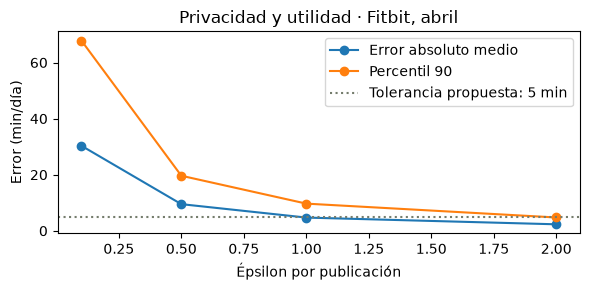
\includegraphics[width=0.75\textwidth]{privacidad-utilidad-fitbit.png}
\caption{El error cae rápido hasta $\varepsilon = 1$ y a partir de ahí mejora poco. $\varepsilon = 1$ es el menor valor que cumple la tolerancia de 5 minutos.}
\end{figure}

\textbf{Interpretación:}
\begin{itemize}[nosep]
  \item Con $\varepsilon = 1$, una publicación típica se desvía unos \textbf{5 minutos de 34 ($\approx$\,14\,\%)}. Basta para ver si la actividad del grupo sube o baja, pero \textbf{no} para tomar decisiones sobre una persona. Por eso la interfaz muestra la unidad y el periodo de cada estimación.
  \item Con $\varepsilon = 0{,}1$ se omite el resultado en el 16\,\% de los casos y el error es de casi la misma magnitud que la media: más privacidad, pero la estadística deja de ser útil.
  \item La protección tiene \textbf{otros costos además del ruido}. Acotar la contribución de cada persona baja la referencia de 34,69 a 34,05 min/día y subestima a las personas más activas. Dar un voto por persona, en vez de uno por fila (35,49), también cambia la cifra. Lo documentamos en vez de ocultarlo.
\end{itemize}

% ---------------------------------------------------------------
\section{Utilidad para modelado}
\label{sec:modelo}

Para medir el efecto de la privacidad en un modelo, entrenamos un clasificador sobre Gym que predice si una sesión dura \textbf{al menos 75 minutos}, a partir del nivel de experiencia y la frecuencia semanal. Datos: 681 filas de entrenamiento y 292 de prueba.
\begin{itemize}[nosep]
  \item \textbf{Referencia:} un histograma de 21 combinaciones $\times$ 2 clases.
  \item \textbf{Versión privada:} el mismo histograma con ruido de Laplace (sensibilidad $L_1 = 1$, porque una fila cambia una sola celda), 30 entrenamientos por cada $\varepsilon$. Aquí la unidad protegida es \textbf{una fila}, porque Gym no tiene un identificador de persona a lo largo del tiempo.
\end{itemize}

\begin{table}[H]
\centering\small
\begin{tabular}{@{}lrr@{}}
\toprule
\textbf{Resultado en prueba} & \textbf{Sin protección} & \textbf{Con $\varepsilon = 1$ (media de 30)} \\
\midrule
Exactitud & 70,9\,\% & 68,4\,\% \\
Exactitud balanceada & 69,4\,\% & 68,8\,\% \\
AUC del ataque de inferencia de membresía & 0,492 & 0,493 \\
Exactitud, grupo femenino ($n = 128$) & 71,1\,\% & 68,0\,\% \\
Exactitud, grupo masculino ($n = 164$) & 70,7\,\% & 68,7\,\% \\
\bottomrule
\end{tabular}
\caption{Clasificador de duración de sesión en Gym, con y sin privacidad diferencial.}
\end{table}

\begin{figure}[H]
\centering
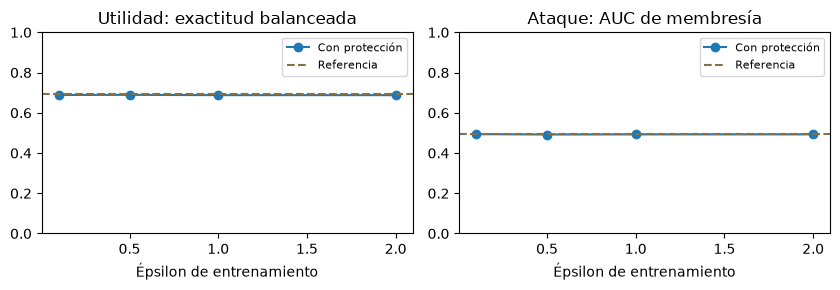
\includegraphics[width=0.9\textwidth]{modelo-gym.png}
\caption{La exactitud balanceada y el ataque de membresía casi no cambian con $\varepsilon$.}
\end{figure}

\textbf{Interpretación:}
\begin{itemize}[nosep]
  \item \textbf{El costo en utilidad es bajo:} $-2{,}5$ puntos de exactitud y $-0{,}6$ de exactitud balanceada.
  \item \textbf{El ataque de membresía \cite{shokri2017} no funciona en ninguna de las dos versiones} (AUC $\approx 0{,}49$, o sea, azar). Un modelo de 42 conteos casi no memoriza filas individuales, así que en este caso \textbf{no pudimos demostrar empíricamente} que la privacidad diferencial reduzca el riesgo. La garantía sigue siendo la matemática de la sección~\ref{sec:dp}.
  \item \textbf{Limitación detectada:} con $\varepsilon = 1$ y $\varepsilon = 2$ los resultados son idénticos. El experimento usa la misma semilla para cada $\varepsilon$, de modo que el ruido tiene siempre el mismo signo. La caída viene de unas pocas celdas casi empatadas que el ruido voltea sin importar su tamaño. Un experimento más sólido debería usar semillas independientes por $\varepsilon$.
\end{itemize}

% ---------------------------------------------------------------
\section{Evaluación de impacto (DPIA)}
\label{sec:dpia}

\subsection{Descripción del tratamiento}
\begin{table}[H]
\centering\small
\begin{tabularx}{\textwidth}{@{}p{3.3cm}Y@{}}
\toprule
\textbf{Elemento} & \textbf{Detalle} \\
\midrule
Responsable & Alzace Fitness (el club). El entrenador actúa solo sobre sus clientes asignados. El operador técnico custodia las claves, los respaldos y el presupuesto $\varepsilon$. \\
Encargados previstos & Supabase (base de datos y autenticación) y Render (API y web) para el despliegue. \\
Titulares & Clientes del entrenamiento virtual. En la demo son personas ficticias; los participantes de Fitbit son datos de estudio. \\
Datos & Identificación (nombre, correo), actividad diaria, sueño, frecuencia cardíaca, peso y \% de grasa, metas y sesiones. \\
Categoría legal & \textbf{Datos sensibles (salud)} según la Ley 29733: exigen consentimiento \textbf{por escrito} y medidas de seguridad reforzadas. \\
Finalidad principal & Acompañar el entrenamiento que el cliente solicitó. \\
Finalidad secundaria & Estimar tendencias grupales de actividad. Es \textbf{opcional}: requiere consentimiento propio y empieza desactivada. \\
\bottomrule
\end{tabularx}
\end{table}

\subsection{Necesidad y proporcionalidad}
\begin{itemize}[nosep]
  \item \textbf{Minimización:} la estadística grupal usa solo los minutos activos, no el peso ni la frecuencia cardíaca. El panel de administración \textbf{no muestra} historias biométricas.
  \item \textbf{Limitación de la finalidad:} el permiso de un estudio no autoriza a contactar a sus participantes ni a convertirlos en clientes. Los datos de Fitbit solo alimentan la estadística del estudio.
  \item \textbf{Base legal:} el seguimiento individual se basa en la relación con el servicio y en el consentimiento expreso para datos de salud. La analítica grupal se basa en un consentimiento \textbf{separado y revocable}. Negarse no afecta el acceso al plan.
  \item \textbf{Alternativa menos invasiva:} se descartó el vínculo Fitbit--Gym, porque crearía perfiles inexistentes sin ningún beneficio para el titular.
\end{itemize}

\subsection{Riesgos a lo largo del ciclo de vida}
Probabilidad (P) $\times$ impacto (I): A = alto, M = medio, B = bajo. La categoría sigue LINDDUN \cite{linddun}.

\begin{table}[H]
\centering\small
\begin{tabularx}{\textwidth}{@{}lp{1.9cm}Yp{2.6cm}ccc@{}}
\toprule
\textbf{\#} & \textbf{Etapa} & \textbf{Escenario de riesgo} & \textbf{LINDDUN} & \textbf{P} & \textbf{I} & \textbf{Inicial} \\
\midrule
R1 & Acceso & Un entrenador o cliente consulta la ficha de otro cliente (IDOR) & Disclosure & M & A & \textbf{Alto} \\
R2 & Estadística & Comparar promedios publicados permite reconocer la rutina de una persona & Linkability, Identifiability & M & A & \textbf{Alto} \\
R3 & Estadística & Republicar el mismo mes con ruido nuevo hasta promediarlo & Disclosure & M & A & \textbf{Alto} \\
R4 & Recolección & Participar en la estadística se percibe como condición del servicio & Non-compliance, Unawareness & M & A & \textbf{Alto} \\
R5 & Conservación & Robo de la base o de un respaldo con datos de salud en claro & Disclosure & M & A & \textbf{Alto} \\
R6 & Preparación & Fechas y patrones de actividad permiten reidentificar a pesar del seudónimo & Linkability & M & M & Medio \\
R7 & Uso & Una predicción sesgada cambia el plan de una persona & Ética: sesgo & M & A & \textbf{Alto} \\
R8 & Estadística & Personas con pocos días quedan subrepresentadas, o el tope subestima a las muy activas & Ética: sesgo & A & B & Medio \\
R9 & Respaldo & Restaurar un respaldo antiguo ``devuelve'' presupuesto ya gastado & Disclosure & B & A & Medio \\
\bottomrule
\end{tabularx}
\caption{Riesgos identificados.}
\end{table}

\subsection{Medidas y riesgo residual}
\begin{table}[H]
\centering\small
\begin{tabularx}{\textwidth}{@{}lYp{4.4cm}c@{}}
\toprule
\textbf{\#} & \textbf{Medida implementada} & \textbf{Cómo se verifica} & \textbf{Residual} \\
\midrule
R1 & La API autoriza \textbf{cada objeto} por rol y por propietario, y audita las denegaciones. & Probado: el cliente recibe 403 al pedir la ficha de otro; el entrenador recibe 403 con un cliente no asignado. & Bajo \\
R2 & Privacidad diferencial $\varepsilon = 1$ a nivel de persona, aporte acotado y umbral sobre el conteo con ruido. & Prueba de sensibilidad y experimento de 300 simulaciones. & Medio \\
R3 & Presupuesto global $\varepsilon = 2$, cargo y publicación en la misma transacción, resultado guardado. & Probado: publicar dos veces devuelve el mismo valor y no gasta más $\varepsilon$. & Bajo \\
R4 & Pantalla de consentimiento con el propósito explicado, opción desactivada por defecto, retiro y registro de la preferencia. & Recorrido en ``Mi privacidad''. & Bajo \\
R5 & Cifrado AES-256-GCM por campo, con datos asociados (tabla, propietario, fecha, versión de clave). Respaldo cifrado con otra clave. Rotación de claves. & Una manipulación invalida el descifrado. Pruebas de respaldo y verificación. & Medio \\
R6 & Seudónimo HMAC con clave separada. Los CSV originales quedan fuera de Git y de los paneles. & Revisión del repositorio y \texttt{.gitignore}. & Medio \\
R7 & El modelo se queda en el notebook (laboratorio). Revisión humana obligatoria y comparación de utilidad por grupo. & Sección~\ref{sec:modelo}. & Bajo \\
R8 & Promedio por persona. El efecto del tope se cuantifica y se publica (34,69 $\rightarrow$ 34,05). & Sección~\ref{sec:dp}. & Medio \\
R9 & Antes de una nueva publicación se concilia el último historial. Si falta, se bloquean las publicaciones. & Procedimiento de recuperación. & Medio \\
\bottomrule
\end{tabularx}
\caption{Medidas y riesgo residual.}
\end{table}

\subsection{Decisión}
\textbf{Se puede pilotar con condiciones.} Ningún riesgo residual queda en nivel alto. Antes de incorporar clientes reales hay que:
\begin{enumerate}[nosep]
  \item desplegar con TLS en ambos extremos (Supabase y Render);
  \item definir un plazo de conservación y una vía de eliminación verificable, incluidas las copias;
  \item designar a quién atiende las solicitudes ARCO;
  \item inscribir el banco de datos ante la ANPD;
  \item ensayar un incidente con el equipo (notificación en 48 h, D.S. 016-2024-JUS).
\end{enumerate}

% ---------------------------------------------------------------
\section{Reflexiones éticas}

\subsection*{Sesgo algorítmico}
\begin{itemize}[nosep]
  \item La privacidad diferencial \textbf{no afecta a todos por igual}. La exactitud del grupo femenino cayó 3,1 puntos y la del masculino 2,0, así que la brecha pasó de 0,4 a 0,7 puntos. Es el efecto que describen Bagdasaryan et al. \cite{bagdasaryan2019}: el ruido perjudica más a los grupos con menos datos.
  \item Las categorías de género del dataset (solo dos) dejan fuera otras identidades. El tamaño de los grupos tampoco permite conclusiones fuertes.
  \item \textbf{``Un día sin reloj no es un día inactivo''.} Por eso la adherencia se calcula con sesiones declaradas como cumplidas, no con días sin registro. Si no, se castigaría a quien no tiene un wearable.
\end{itemize}

\subsection*{Transparencia}
\begin{itemize}[nosep]
  \item Publicamos el método, la unidad protegida, el $\varepsilon$ y el error esperado (sección~\ref{sec:dp}), incluidos los costos del tope y del voto por persona.
  \item La interfaz presenta cada estadística con su unidad y su periodo. Así se evita que alguien la lea como un dato individual.
\end{itemize}

\subsection*{Consentimiento}
\begin{itemize}[nosep]
  \item El consentimiento para la analítica es \textbf{separado, opcional, desactivado por defecto y revocable}. El cliente no pierde su plan si se niega.
  \item Retirarlo afecta a las consultas futuras, pero \textbf{no borra} lo ya publicado. Lo explicamos en la pantalla, porque un consentimiento solo es informado si la persona sabe qué no se puede deshacer.
\end{itemize}

\subsection*{Tensión de fondo}
Más privacidad ($\varepsilon$ pequeño) da una estadística inútil para el club. Menos privacidad expone a las personas. Elegimos $\varepsilon = 1$ con un criterio de utilidad \textbf{fijado antes} de mirar los resultados, y limitamos el número de publicaciones. La decisión se puede revisar, pero queda documentada y no es arbitraria.

% ---------------------------------------------------------------
\section{Seguridad y verificación}

\begin{table}[H]
\centering\small
\begin{tabularx}{\textwidth}{@{}p{3cm}Y@{}}
\toprule
\textbf{Medida} & \textbf{Implementación} \\
\midrule
Cifrado en reposo & AES-256-GCM por campo, nonce de 96 bits y etiqueta autenticada. \\
Contraseñas & bcrypt con coste 12 y sal individual. En el modo alojado, Supabase Auth. \\
Sesiones & Cookie HttpOnly y SameSite=Strict (Secure en el modo alojado). Verificación del origen y de un encabezado propio en las escrituras. \\
Autorización & Por rol y por registro, validada en el servidor. \\
Auditoría & Eventos de solo inserción: sesiones, publicaciones, importaciones, denegaciones. \\
Respaldos & Copia cifrada con una clave distinta y verificación por restauración en memoria. \\
En tránsito & En el modo alojado la configuración \textbf{exige} HTTPS y \texttt{sslmode=verify-full} hacia PostgreSQL. Si falta, no arranca. \\
Escaneo & OWASP ZAP 2.17 pasivo con los 4 roles: 38 mensajes y \textbf{solo 3 alertas informativas}, ninguna de riesgo bajo, medio o alto. \\
\bottomrule
\end{tabularx}
\caption{Medidas de seguridad implementadas.}
\end{table}

\textbf{Pruebas ejecutadas} (12/11/2026, en un equipo del grupo con Windows y Python 3.13):
\begin{itemize}[nosep]
  \item \texttt{pytest}: \textbf{8 pruebas pasan}. 1 se omite porque requiere una base PostgreSQL de pruebas, definida en la variable \texttt{ALZACE\_TEST\_PG}.
  \item Next.js compila en modo producción.
  \item Los 3 notebooks se ejecutan de principio a fin, y el experimento reproduce exactamente los resultados guardados en \texttt{evidence/experimentos.json}.
  \item Recorrido en vivo por la API: acceso cruzado denegado (403); escritura sin encabezado propio rechazada (403); publicación repetida sin gasto adicional de $\varepsilon$; evento de auditoría de la publicación registrado (\texttt{estadistica.\allowbreak publicar}).
\end{itemize}

% ---------------------------------------------------------------
\section{Cumplimiento de requerimientos}
\label{sec:cumplimiento}

\begin{table}[H]
\centering\small
\begin{tabularx}{\textwidth}{@{}p{6cm}cY@{}}
\toprule
\textbf{Requerimiento del enunciado final} & \textbf{Estado} & \textbf{Evidencia} \\
\midrule
Evaluar riesgos de privacidad y éticos & Cumplido & Secciones \ref{sec:dpia} y 8 \\
Mantener la utilidad para análisis y modelado & Cumplido & Error de 4,7 min; $-2{,}5$ puntos de exactitud \\
Implementar y evaluar privacidad diferencial & Cumplido & Sección~\ref{sec:dp}, \texttt{backend/privacy.py}, notebook 02 \\
Justificar la librería y $\varepsilon$ con evidencia & Cumplido & Secciones 5.4 y 5.5, referencias \\
DPIA del ciclo de vida & Cumplido & Sección~\ref{sec:dpia} \\
Ética: sesgo, transparencia y consentimiento & Cumplido & Sección 8 \\
Al menos una base de datos & Cumplido & SQLite (demo) y PostgreSQL (modo alojado) \\
Front y backend & Cumplido & Next.js y FastAPI \\
Notebooks & Cumplido & \texttt{notebooks/01--03} \\
\bottomrule
\end{tabularx}
\caption{Cumplimiento del enunciado final.}
\end{table}

\textbf{Lo que no se logró y por qué:}
\begin{table}[H]
\centering\small
\begin{tabularx}{\textwidth}{@{}p{5cm}Y@{}}
\toprule
\textbf{Pendiente} & \textbf{Justificación} \\
\midrule
Despliegue en Supabase + Render con TLS (prometido en el parcial) & La configuración está lista y exige HTTPS y \texttt{verify-full}, pero no llegamos a validar el staging con cuentas del equipo a tiempo. La demo es local, por eso \textbf{no evaluamos TLS en producción}. \\
Prueba de concurrencia sobre PostgreSQL & Existe (\texttt{tests/test\_postgres.py}), pero necesita una base de pruebas externa. Se omitió en esta ejecución. \\
Escaneo ZAP activo & Solo se ejecutó el pasivo. El activo debe hacerse con autorización sobre el staging. \\
Plazo de conservación y eliminación verificable & Está planteado en la DPIA y es condición antes del piloto. \\
\bottomrule
\end{tabularx}
\end{table}

% ---------------------------------------------------------------
\section{Conclusiones}
\begin{enumerate}[nosep]
  \item \textbf{La privacidad diferencial es viable para la estadística del club.} Con $\varepsilon = 1$, el error típico es de unos 5 minutos sobre 34, suficiente para ver tendencias sin exponer a nadie. El valor de $\varepsilon$ se eligió con un criterio fijado antes del experimento.
  \item \textbf{El costo para el modelado fue bajo} ($-2{,}5$ puntos), pero \textbf{no neutral}: aumentó un poco la brecha entre grupos. Proteger la privacidad y ser justo con todos los grupos son objetivos que hay que medir por separado.
  \item \textbf{La privacidad no es solo ruido.} Las decisiones que más protegen fueron de diseño: la unidad protegida (la persona), el presupuesto con resultados guardados, el consentimiento separado, no mostrar datos individuales al administrador y descartar un vínculo de datos sin fundamento.
  \item \textbf{Lo que falta es operativo:} despliegue con TLS, conservación y ARCO. Por eso la decisión de la DPIA es ``pilotar con condiciones'', no ``lanzar''.
\end{enumerate}

% ---------------------------------------------------------------
\section{Lecciones aprendidas y retrospectiva}
\label{sec:lecciones}
\begin{itemize}[nosep]
  \item \textbf{Cambiar el diseño cuando los datos no lo sostienen.} En el parcial propusimos unir Fitbit y Gym al azar. Al implementarlo vimos que generaba personas inexistentes, así que lo descartamos y analizamos cada fuente por separado.
  \item \textbf{Definir la unidad protegida es lo más difícil.} Proteger ``una fila'' o ``una persona'' cambia la sensibilidad y la garantía. En Fitbit pudimos proteger a la persona; en Gym, solo la fila.
  \item \textbf{Un experimento también puede tener errores de diseño.} Usar la misma semilla para todos los $\varepsilon$ hizo indistinguibles $\varepsilon = 1$ y $\varepsilon = 2$ en el modelo. Lo detectamos al reproducir los resultados.
  \item \textbf{El presupuesto $\varepsilon$ es un recurso que se acaba.} Durante las pruebas gastamos la mitad del presupuesto de la demo y tuvimos que reiniciar la base antes de presentarla. En un servicio real, esto obliga a planificar qué preguntas valen la pena.
  \item \textbf{Retrospectiva de equipo.} La implementación avanzó en un solo repositorio, y la verificación, el informe y la presentación se cerraron al final. Para otro proyecto, conviene revisar entregables y código en paralelo desde el inicio, y no concentrar la documentación en la última semana.
\end{itemize}

% ---------------------------------------------------------------
\begin{thebibliography}{9}
\bibitem{dwork2014} C. Dwork y A. Roth. \emph{The Algorithmic Foundations of Differential Privacy}. Foundations and Trends in Theoretical Computer Science, 2014.
\bibitem{holohan2019} N. Holohan, S. Braghin, P. Mac Aonghusa y K. Levacher. \emph{Diffprivlib: The IBM Differential Privacy Library}. 2019. \url{https://arxiv.org/abs/1907.02444}
\bibitem{holohan2021} N. Holohan y S. Braghin. \emph{Secure Random Sampling in Differential Privacy}. 2021. \url{https://arxiv.org/abs/2107.10138}
\bibitem{nist800226} NIST. \emph{SP 800-226: Guidelines for Evaluating Differential Privacy Guarantees}. 2025. \url{https://csrc.nist.gov/pubs/sp/800/226/final}
\bibitem{bagdasaryan2019} E. Bagdasaryan, O. Poursaeed y V. Shmatikov. \emph{Differential Privacy Has Disparate Impact on Model Accuracy}. NeurIPS, 2019.
\bibitem{shokri2017} R. Shokri, M. Stronati, C. Song y V. Shmatikov. \emph{Membership Inference Attacks Against Machine Learning Models}. IEEE S\&P, 2017.
\bibitem{ley29733} Ley N.\textdegree{}~29733, Ley de Protección de Datos Personales, y su reglamento D.S. 016-2024-JUS.
\bibitem{linddun} LINDDUN: privacy threat modeling framework. \url{https://linddun.org}
\bibitem{zap} OWASP ZAP. \url{https://www.zaproxy.org}
\end{thebibliography}

\end{document}
